\subsection{Building a Base Multiplier} \label{sec_build_base_mult}

%% here explain the algorithm and its caveats and why it is not always a square area. 

% Explain the tiling algorithm and how it works (cite Roy et al.~\cite{royTileMultiplicationEfficient2014})
To construct large multipliers efficiently on FPGAs, we build a base multiplier using a tiling algorithm inspired by Roy et al.~\cite{royTileMultiplicationEfficient2014}.
Given DSP primitive dimensions $W_1\times W_2$ (e.g., $26\times17$ for DSP48E2), the algorithm chooses integers $n,m$ so that the covered width
\[
\bar{M} \geq n \cdot  W_1  + m \cdot W_2 .
\]
Tiles of size $W_1\times W_2$ and $W_2\times W_1$ are placed along the boundary of a $\bar{M}\times\bar{M}$ square, leaving a smaller square region in the middle that is recursively tiled.
However, the original algorithm has practical limitations that our work addresses:
\begin{itemize}
    \item The remaining middle region is not guaranteed to be a square for arbitrary $n,m$.
    \item Hardware mapping is not architecture-aware (e.g., cascade/shift constraints), and it does not explicitly provide variants that trade off LUT usage and latency.
\end{itemize}

To guarantee a square remaining middle region, we constrain one coefficient to 1 (either $n=1$ or $m=1$).
% DSP slices covering MSB regions can use the full signed range ($27\times18$), while LSB-only regions must use the unsigned range ($26\times17$). 
% Therefore, a tiling yields either an $(n\cdot26+m\cdot17)$-bit unsigned multiplier or an $(n\cdot26+m\cdot17+1)$-bit signed multiplier.
Figure ~\ref{fig_tiling_examples} shows the tiling scheme for two different multiplier sizes, $44\times44$ and $78\times78$ signed multipliers.
To address the remaining issues, we separate generating multiplication terms (tiles) from mapping those terms onto DSP slices.
This enables architecture-aware mapping (cascade/shift constraints) and optimization for either LUT minimization or latency.
Figure~\ref{fig_grouping_strategies} compares two mapping strategies.
First, the one-group strategy (Figure~\ref{fig_one_group}) chains as many terms (sorted ascendingly based on their shift amount) as possible to minimize LUTs. 
This ordering allows for non-overlapping bit extraction and keeps additions within the 48-bit limit.
The multi-group strategy (Figure~\ref{fig_three_groups}) forms independent chains whose terms are shifted apart by 17 bits, maximizing cascade usage and enabling parallel evaluation to reduce latency.

\begin{figure}[t]
    \centering
    \begin{subfigure}{0.48\columnwidth}
        \centering
        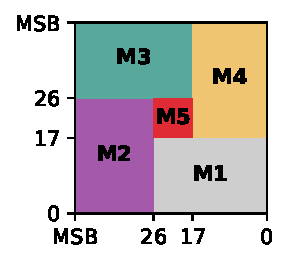
\includegraphics[width=\textwidth]{figures/base_tiling/Tiling_RectFig44x44.pdf}
        \caption{$44\times44$-bit multiplier tiling (5 DSP48E2 blocks).}
        \label{fig_tiling44}
    \end{subfigure}%
    \hfill
    \begin{subfigure}{0.48\columnwidth}
        \centering
        
\includegraphics[width=\textwidth]{figures/base_tiling/Tiling_RectFig78x78.pdf}
        \caption{$78\times78$-bit multiplier tiling (14 DSP48E2 blocks).}
        \label{fig_tiling78}
    \end{subfigure}
\caption{Tiling schemes for different multiplier sizes.}
\label{fig_tiling_examples}
\end{figure}

% second problem 

\begin{figure}[t]
    \centering
    \begin{subfigure}{\columnwidth}
        \centering
        
\includegraphics[width=\textwidth]{figures/base_tiling/comb78_one_group.pdf}
        % 
\includegraphics[width=\textwidth]{figures/base_tiling/comb44_one_group.pdf}

        \caption{One group strategy (Minimizing LUTs).}
        \label{fig_one_group}
    \end{subfigure}
    
    \hfill
    
    \begin{subfigure}{\columnwidth}
        \centering
        
\includegraphics[width=\textwidth]{figures/base_tiling/comb78_three_groups.pdf}
        % 
\includegraphics[width=\textwidth]{figures/base_tiling/comb44_two_groups.pdf}

        \caption{Multi-group strategy (Minimizing latency).}
        \label{fig_three_groups}
    \end{subfigure}
    
\caption{Different grouping strategies for tile mapping optimization. Green rectangles denote the number of pipeline stages. Yellow circles denote the number of the least significant bits to be extracted from P. Also they denote right shift operation of the P by the same amount and pass it to C if the P to C path is used.}
\label{fig_grouping_strategies}
\end{figure}

Table ~\ref{table_diff_ways_base_multiplier} compares the resource usage and latency of different base multipliers built using the two grouping strategies for both $44\times44$ and $78\times78$ multipliers.
As shown, the one group strategy uses fewer LUTs but has double the latency, while the three groups strategy reduces latency at the cost of slightly increased FF usage.
The reason for the increased LUT usage in the $78\times78$ one group variant is that some LUTs are used to balance the pipeline stages instead of FF registers. 

% Adjust the column separation (default is 6pt)
% \setlength{\tabcolsep}{7pt}
\begin{table}
\centering
\caption{Comparison of different ways to build base multipliers}
\resizebox{1\linewidth}{!}{
\begin{tabular}{
lccccc
}
\toprule

% \textbf{}&\textbf{Size}&\textbf{LUTs}&\textbf{FFs}&\textbf{DSPs}&\textbf{Latency}&\textbf{\#Wasted DSPs}\\

\textbf{Primitive Strategy}&\textbf{Size}&\textbf{LUTs}&\textbf{FFs}&\textbf{DSPs}&
\shortstack{\textbf{Latency} \\ [-0.5ex] \textbf{(Cycles)}}\\


\midrule
One group&78&537&1051&14&28\\
                     &44&78&323&5&9\\
\midrule
Multi-group&78&429&1386&14&14\\
                        &44&105&334&5&8\\
\bottomrule
\end{tabular}
}
\label{table_diff_ways_base_multiplier}
\end{table}





%% Comparison with the IP multiplier performance 

To test the effectiveness of our base multiplier design, we compare one of our base multipliers against the AMD Vivado IP multiplier.
The AMD Vivado IP block offers a maximum size of $64\times64$ bits and implemented following the design methodology presented in~\cite{xilinxincIPMultiplier2015}.
Our base multiplier matches the IP's maximum frequency, supports larger sizes, and uses 2 fewer DSPs at the cost of extra 210 LUTs.
To contextualize DSP usage, we compute the theoretical minimum number of $26\times17$ tiles for a given size (Equation~\ref{eq_mul_best}).
The $64\times64$ IP design uses around 7 DSPs above this limit, while our primitive-based design only sacrifices a few bits in one slice.
The two designs are compared when tiled to larger sizes using both Schoolbook and Karatsuba decomposition.
% Table ~\ref{table_tilingup_primitive_vs_ip} summarizes the comparison between the two designs when tiled to larger sizes while 
Figure ~\ref{fig_prim64vs77_resources} and Figure ~\ref{fig_prim64vs77_frequency} show the resource usage and maximum frequency comparison respectively.
Our base primitive multiplier consistently uses fewer DSPs and achieves higher frequency across all tiled sizes and decomposition schemes.


\begin{equation} \label{eq_mul_best}
\begin{split}
\text{optimal\_num\_DSPs} &= \frac{(Size \times Size)}{(26 \times 17)}\\ 
% \text{num\_wasted\_DSPs} &=  \text{num\_used\_DSPs} - \text{optimal\_num\_DSPs} \\ 
\end{split}
\end{equation}



\begin{figure}[t]
    \centering
    \begin{subfigure}[t]{\columnwidth}
        \centering
        
\includegraphics[width=\columnwidth]{figures/base_tiling/prim64vs77_combined_lut_ff_dsp.pdf}
        \caption{Resource usage}
        \label{fig_prim64vs77_resources}
    \end{subfigure}%
    \hfill
    \begin{subfigure}[t]{\columnwidth}
        \centering
        
\includegraphics[width=\columnwidth]{figures/base_tiling/prim64vs77_max_frequency.pdf}
    \caption{Maximum frequency}
    \label{fig_prim64vs77_frequency}

    \end{subfigure}
\caption{Resource and frequency comparison between Base 64 and Base 78 multipliers when tiled to larger sizes.}
\label{fig_prim64vs77_comparison}
\end{figure}



% %% we need another table comparing different base multipliers when tiled to a larger multiplier size.
% % Adjust the column separation (default is 6pt)
% % \setlength{\tabcolsep}{7pt}
% \begin{table}
% \centering
% \caption{Comparison of $64\times64$ IP multiplier and our $78\times78$ base multiplier when tiled to unsigned larger multiplier sizes. SB denotes Schoolbook, Karat. denotes Karatsuba.}
% \resizebox{1\linewidth}{!}{
% \begin{tabular}{
% llcccccc
% }
% \toprule


% \textbf{}&\textbf{Tiled Size (Grid)}&\textbf{Scheme}&\textbf{LUTs}&\textbf{FFs}&\textbf{DSPs}&
% \shortstack{\textbf{Freq.} \\ [-0.5ex] \textbf{(MHz)}}&
% \shortstack{\textbf{Latency} \\ [-0.5ex] \textbf{(Cycles)}}\\ 

% \midrule
% Base 64 & $64\times64$ & Base & 219 & 722 & 16 & 899 & 18 \\
%         & $128\times128$ ($2\times2$) & Karat. & 1826 & 5349 & 48 & 933 & 26 \\
%         & $128\times128$ ($2\times2$) & SB & 1272 & 4892 & 64 & 862 & 23 \\
%         & $192\times192$ ($3\times3$) & Karat. & 4320 & 13344 & 96 & 803 & 30 \\
%         & $192\times192$ ($3\times3$) & SB & 3319 & 11658 & 144 & 751 & 27 \\
% \midrule
% Base 78 & $78\times78$ & Base & 429 & 1386 & 14 & 1026 & 14 \\
%         & $154\times154$ ($2\times2$) & Karat. & 3026 & 6444 & 42 & 953 & 28 \\
%         & $154\times154$ ($2\times2$) & SB & 2599 & 5292 & 56 & 870 & 21 \\
%         & $231\times231$ ($3\times3$) & Karat. & 7165 & 15031 & 84 & 860 & 37 \\
%         & $231\times231$ ($3\times3$) & SB & 6674 & 11889 & 126 & 795 & 30 \\

% \bottomrule
% \end{tabular}
% }
% \label{table_tilingup_primitive_vs_ip}
% \end{table}








